\documentclass[12pt, a4paper]{article}  

\usepackage{etex} % расширение классического tex в частности позволяет подгружать гораздо больше пакетов, чем мы и займёмся далее

%%%%%%%%%% Математика %%%%%%%%%%
\usepackage{amsmath,amsfonts,amssymb,amsthm,mathtools} 


%%%%%%%%%%%%%%%%%%%%%%%% Шрифты %%%%%%%%%%%%%%%%%%%%%%%%%%%%%%%%%
\usepackage{fontspec}         % пакет для подгрузки шрифтов
\setmainfont{Arial}   % задаёт основной шрифт документа

\defaultfontfeatures{Mapping=tex-text}

\newfontfamily{\cyrillicfonttt}{Arial}
\newfontfamily{\cyrillicfont}{Arial}
\newfontfamily{\cyrillicfontsf}{Arial}

\usepackage{unicode-math}     % пакет для установки математического шрифта
\setmathfont{Asana Math}      % шрифт для математики

\usepackage{polyglossia}      % Пакет, который позволяет подгружать русские буквы
\setdefaultlanguage{russian}  % Основной язык документа
\setotherlanguage{english}    % Второстепенный язык документа


%%%%%%%%%% Работа с картинками %%%%%%%%%
\usepackage{graphicx}                  % Для вставки рисунков
\usepackage{graphics} 
\graphicspath{{pop-art/},{pictures/}}    % можно указать папки с картинками
\usepackage{wrapfig}                   % Обтекание рисунков и таблиц текстом
\usepackage{subfigure}                 % для создания нескольких рисунков внутри одного
\usepackage{rotating}


%%%%%%%%%% Работа с таблицами %%%%%%%%%%
\usepackage{tabularx}            % новые типы колонок
\usepackage{tabulary}            % и ещё новые типы колонок
\usepackage{array}               % Дополнительная работа с таблицами
\usepackage{longtable}           % Длинные таблицы
\usepackage{multirow}            % Слияние строк в таблице
\usepackage{float}               % возможность позиционировать объекты в нужном месте 
\usepackage{booktabs}            % таблицы как в книгах!  
\renewcommand{\arraystretch}{1.3} % больше расстояние между строками

\DeclareMathOperator{\diag}{diag}  % математический оператор, который описывает диагональную матрицу


%заголовок

\author{Никаноров Иван}
\title{Домашняя работа №2. Задание 1}
\date {\today}

\begin{document}

\maketitle

\newpage

\begin{figure} [H]
 \begin{minipage}[h!]{0.32\linewidth}
  \begin{turn} {-90}
  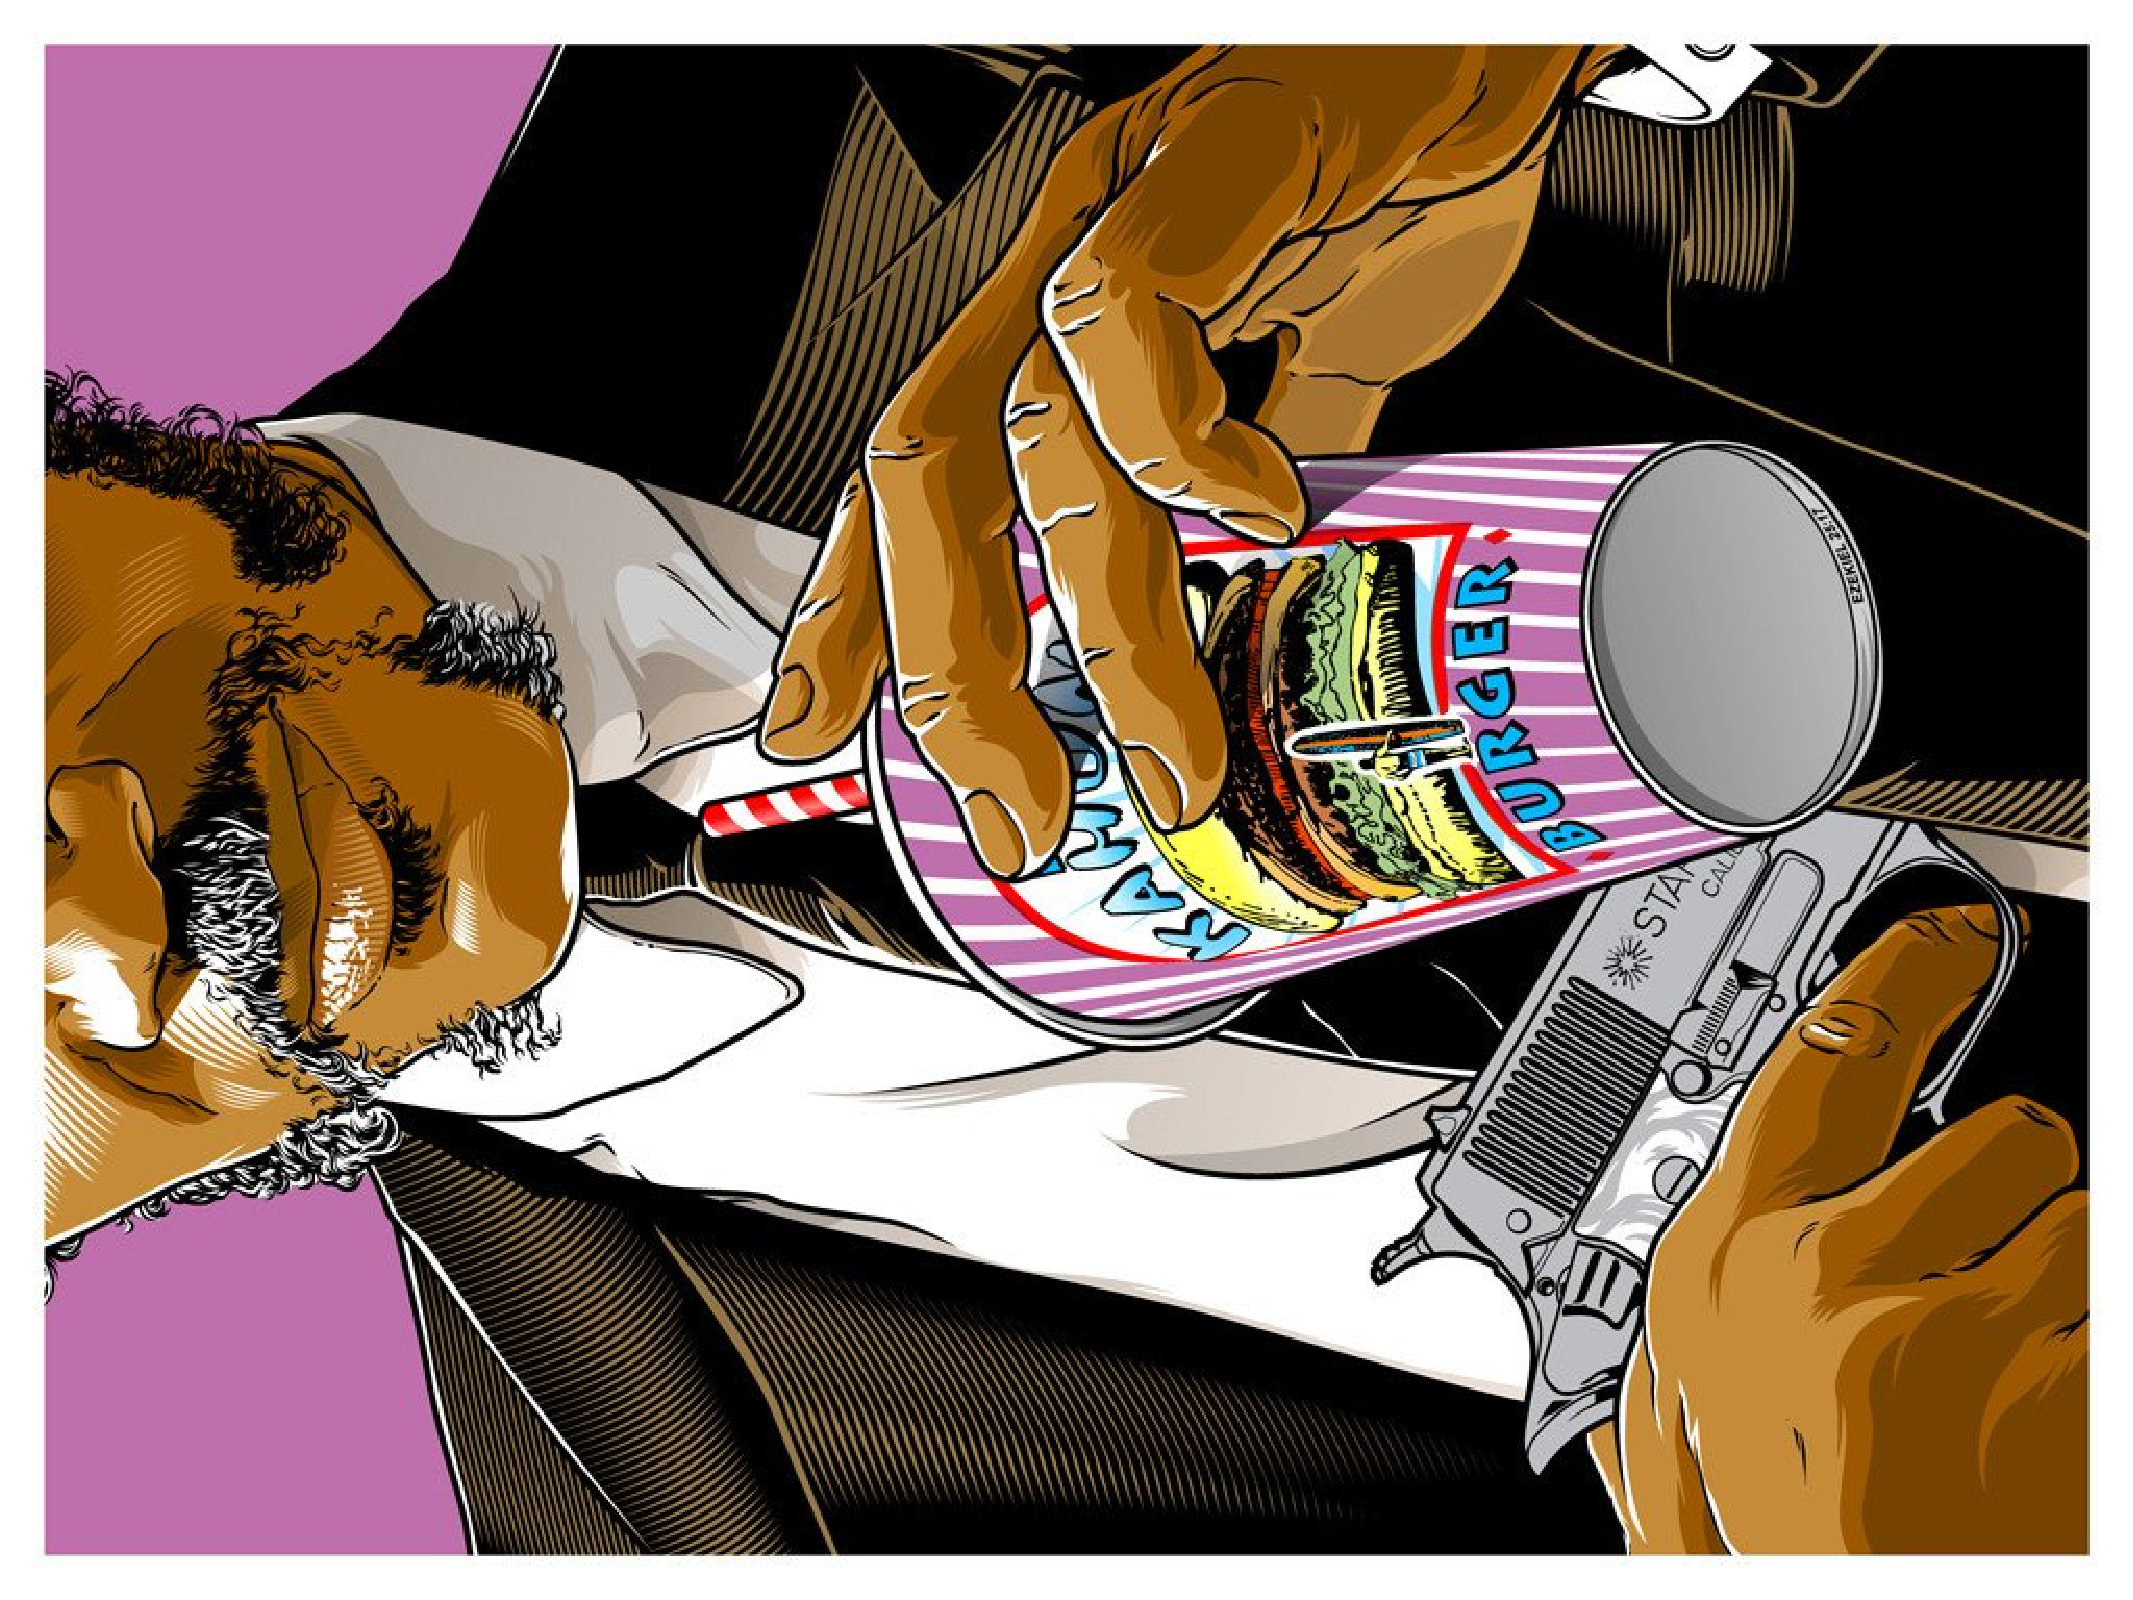
\includegraphics[height=4.3cm, width=10cm, keepaspectratio]{pop1}
  \end{turn}
 \end{minipage}
 \hfill
 \begin{minipage}[h!]{0.32\linewidth}
  
\includegraphics[width=1\linewidth]{pop3}
 \end{minipage}
 \hfill
 \begin{minipage}[h!]{0.32\linewidth}
  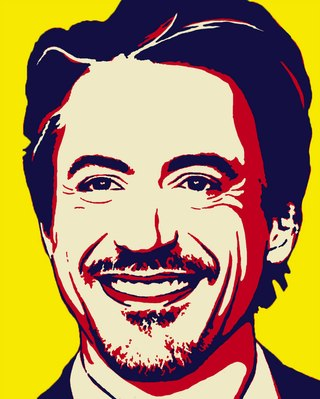
\includegraphics[width=1\linewidth]{pop5}
 \end{minipage}
 \vfill
  \begin{minipage}[h!]{0.32\linewidth}
  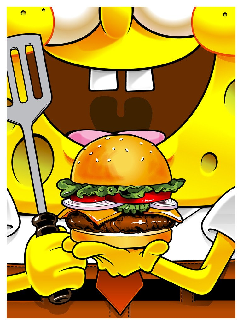
\includegraphics[width=1\linewidth]{pop8}
 \end{minipage}
 \hfill
  \begin{minipage}[h!]{0.32\linewidth}
   \begin{turn} {180}
   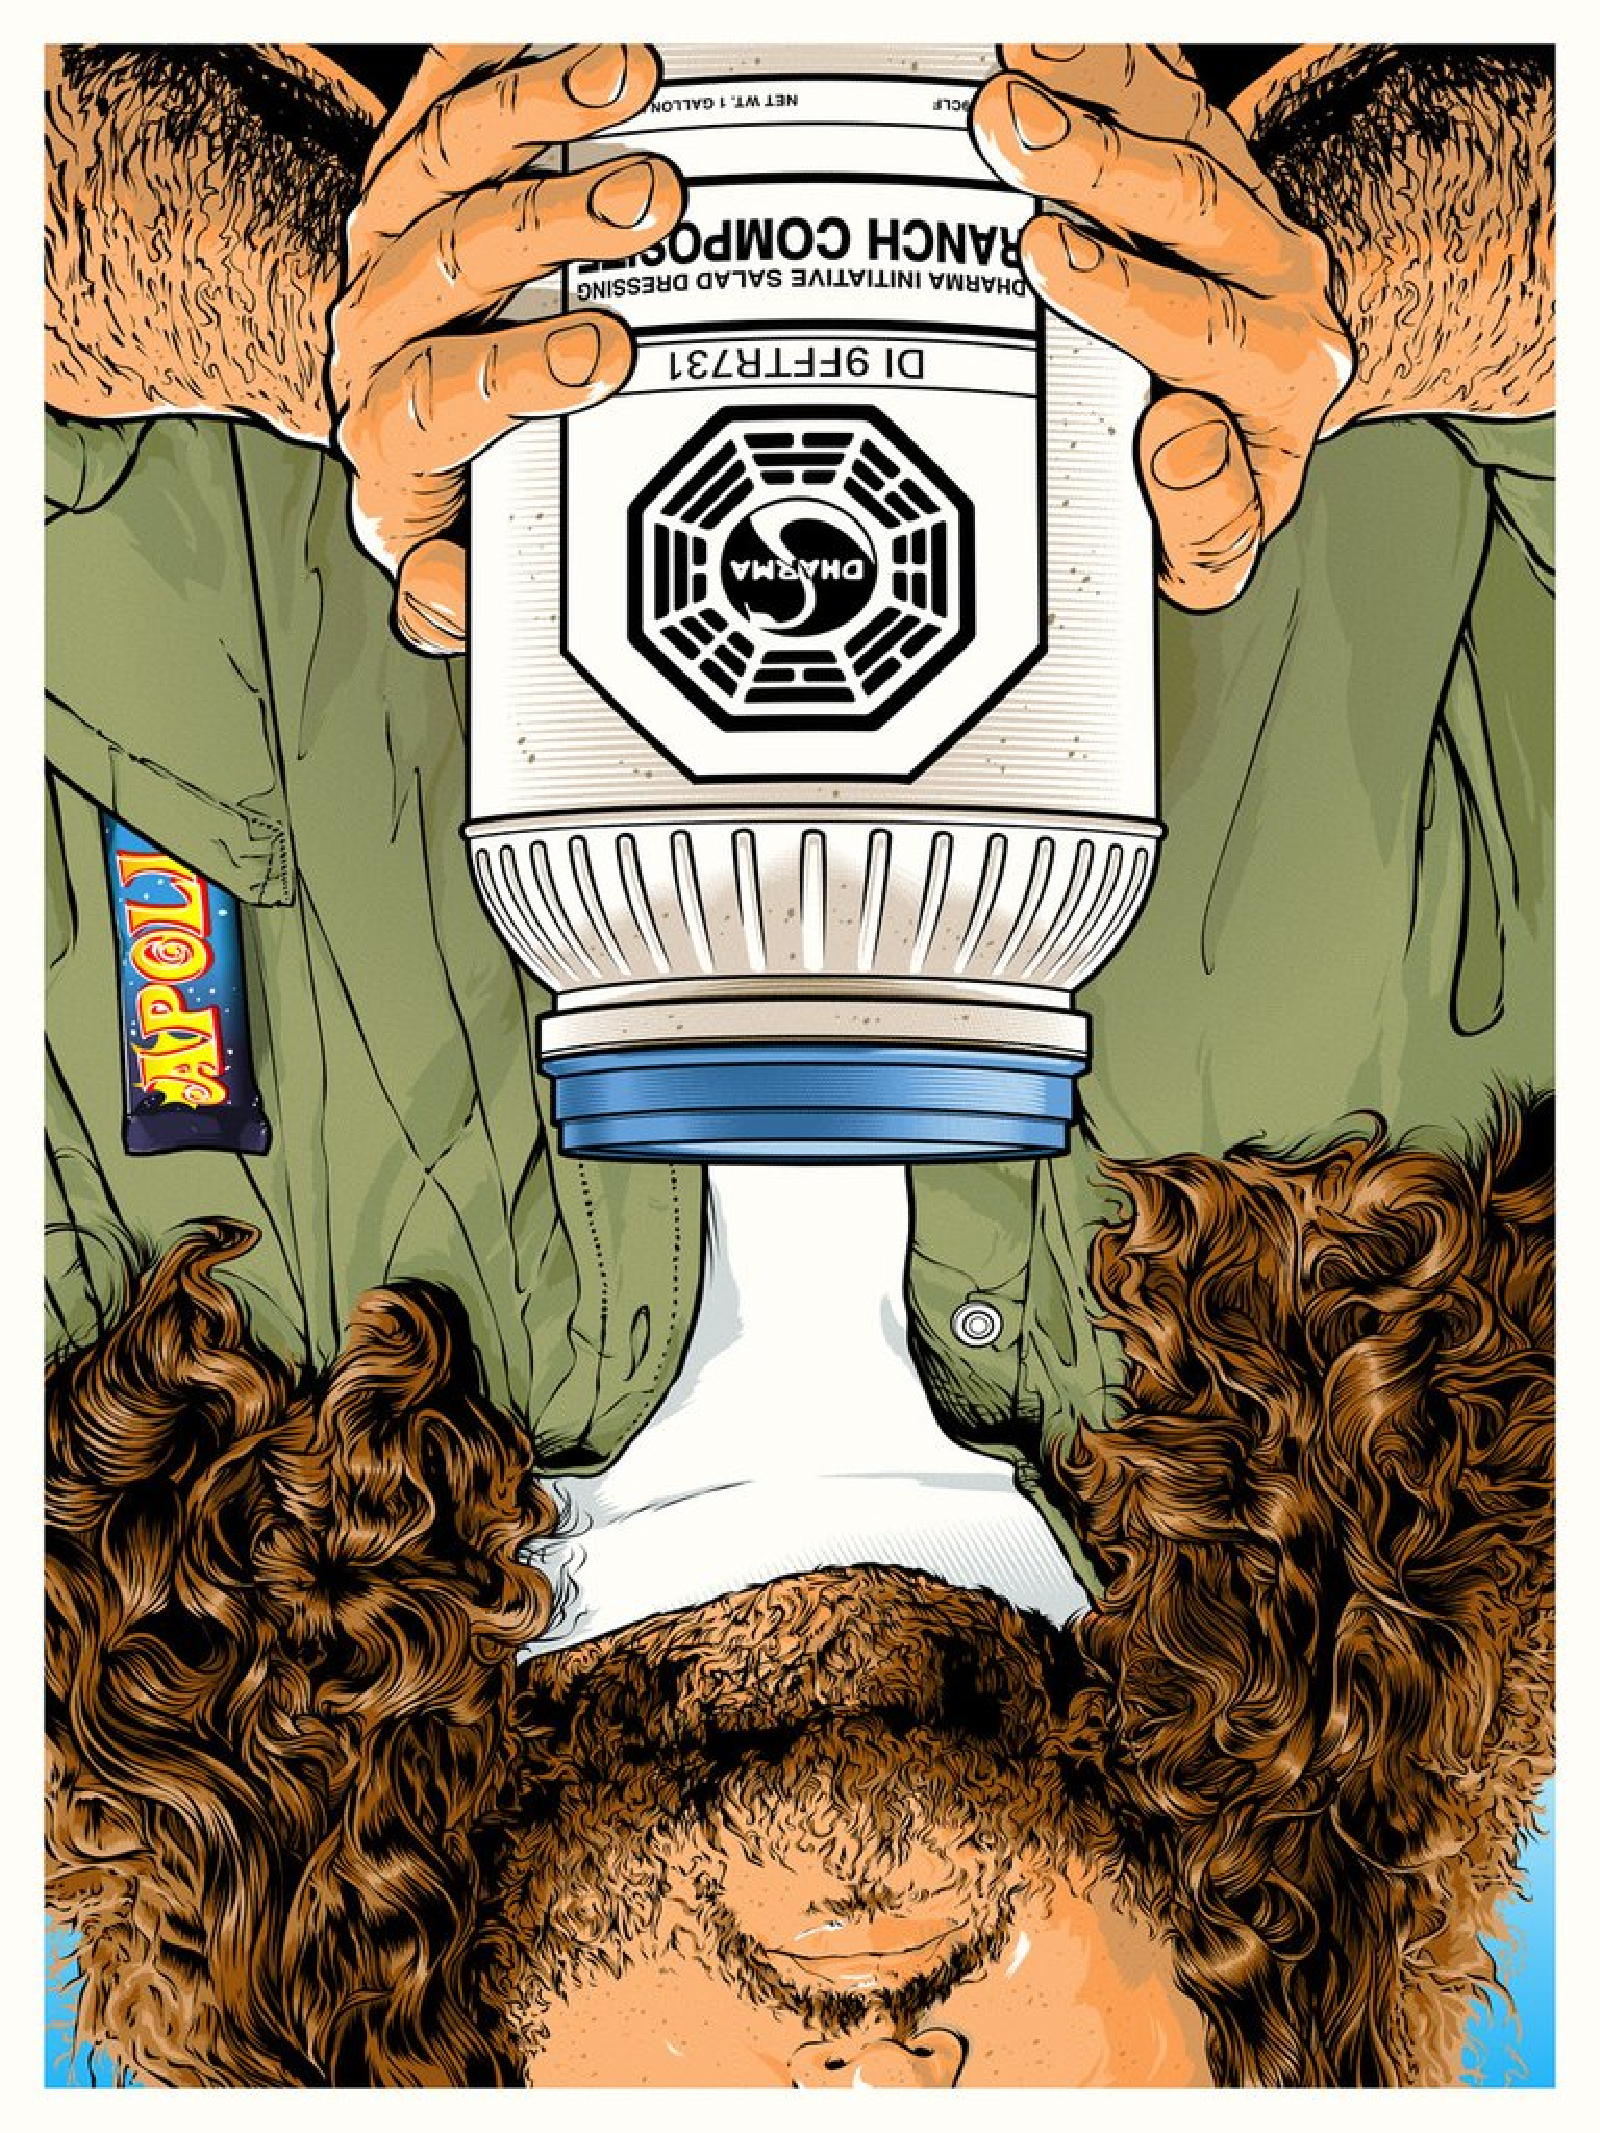
\includegraphics[width=1\linewidth]{pop10}
   \end{turn}
 \end{minipage}
 \hfill
  \begin{minipage}[h!]{0.32\linewidth}
   \begin{turn} {180}
   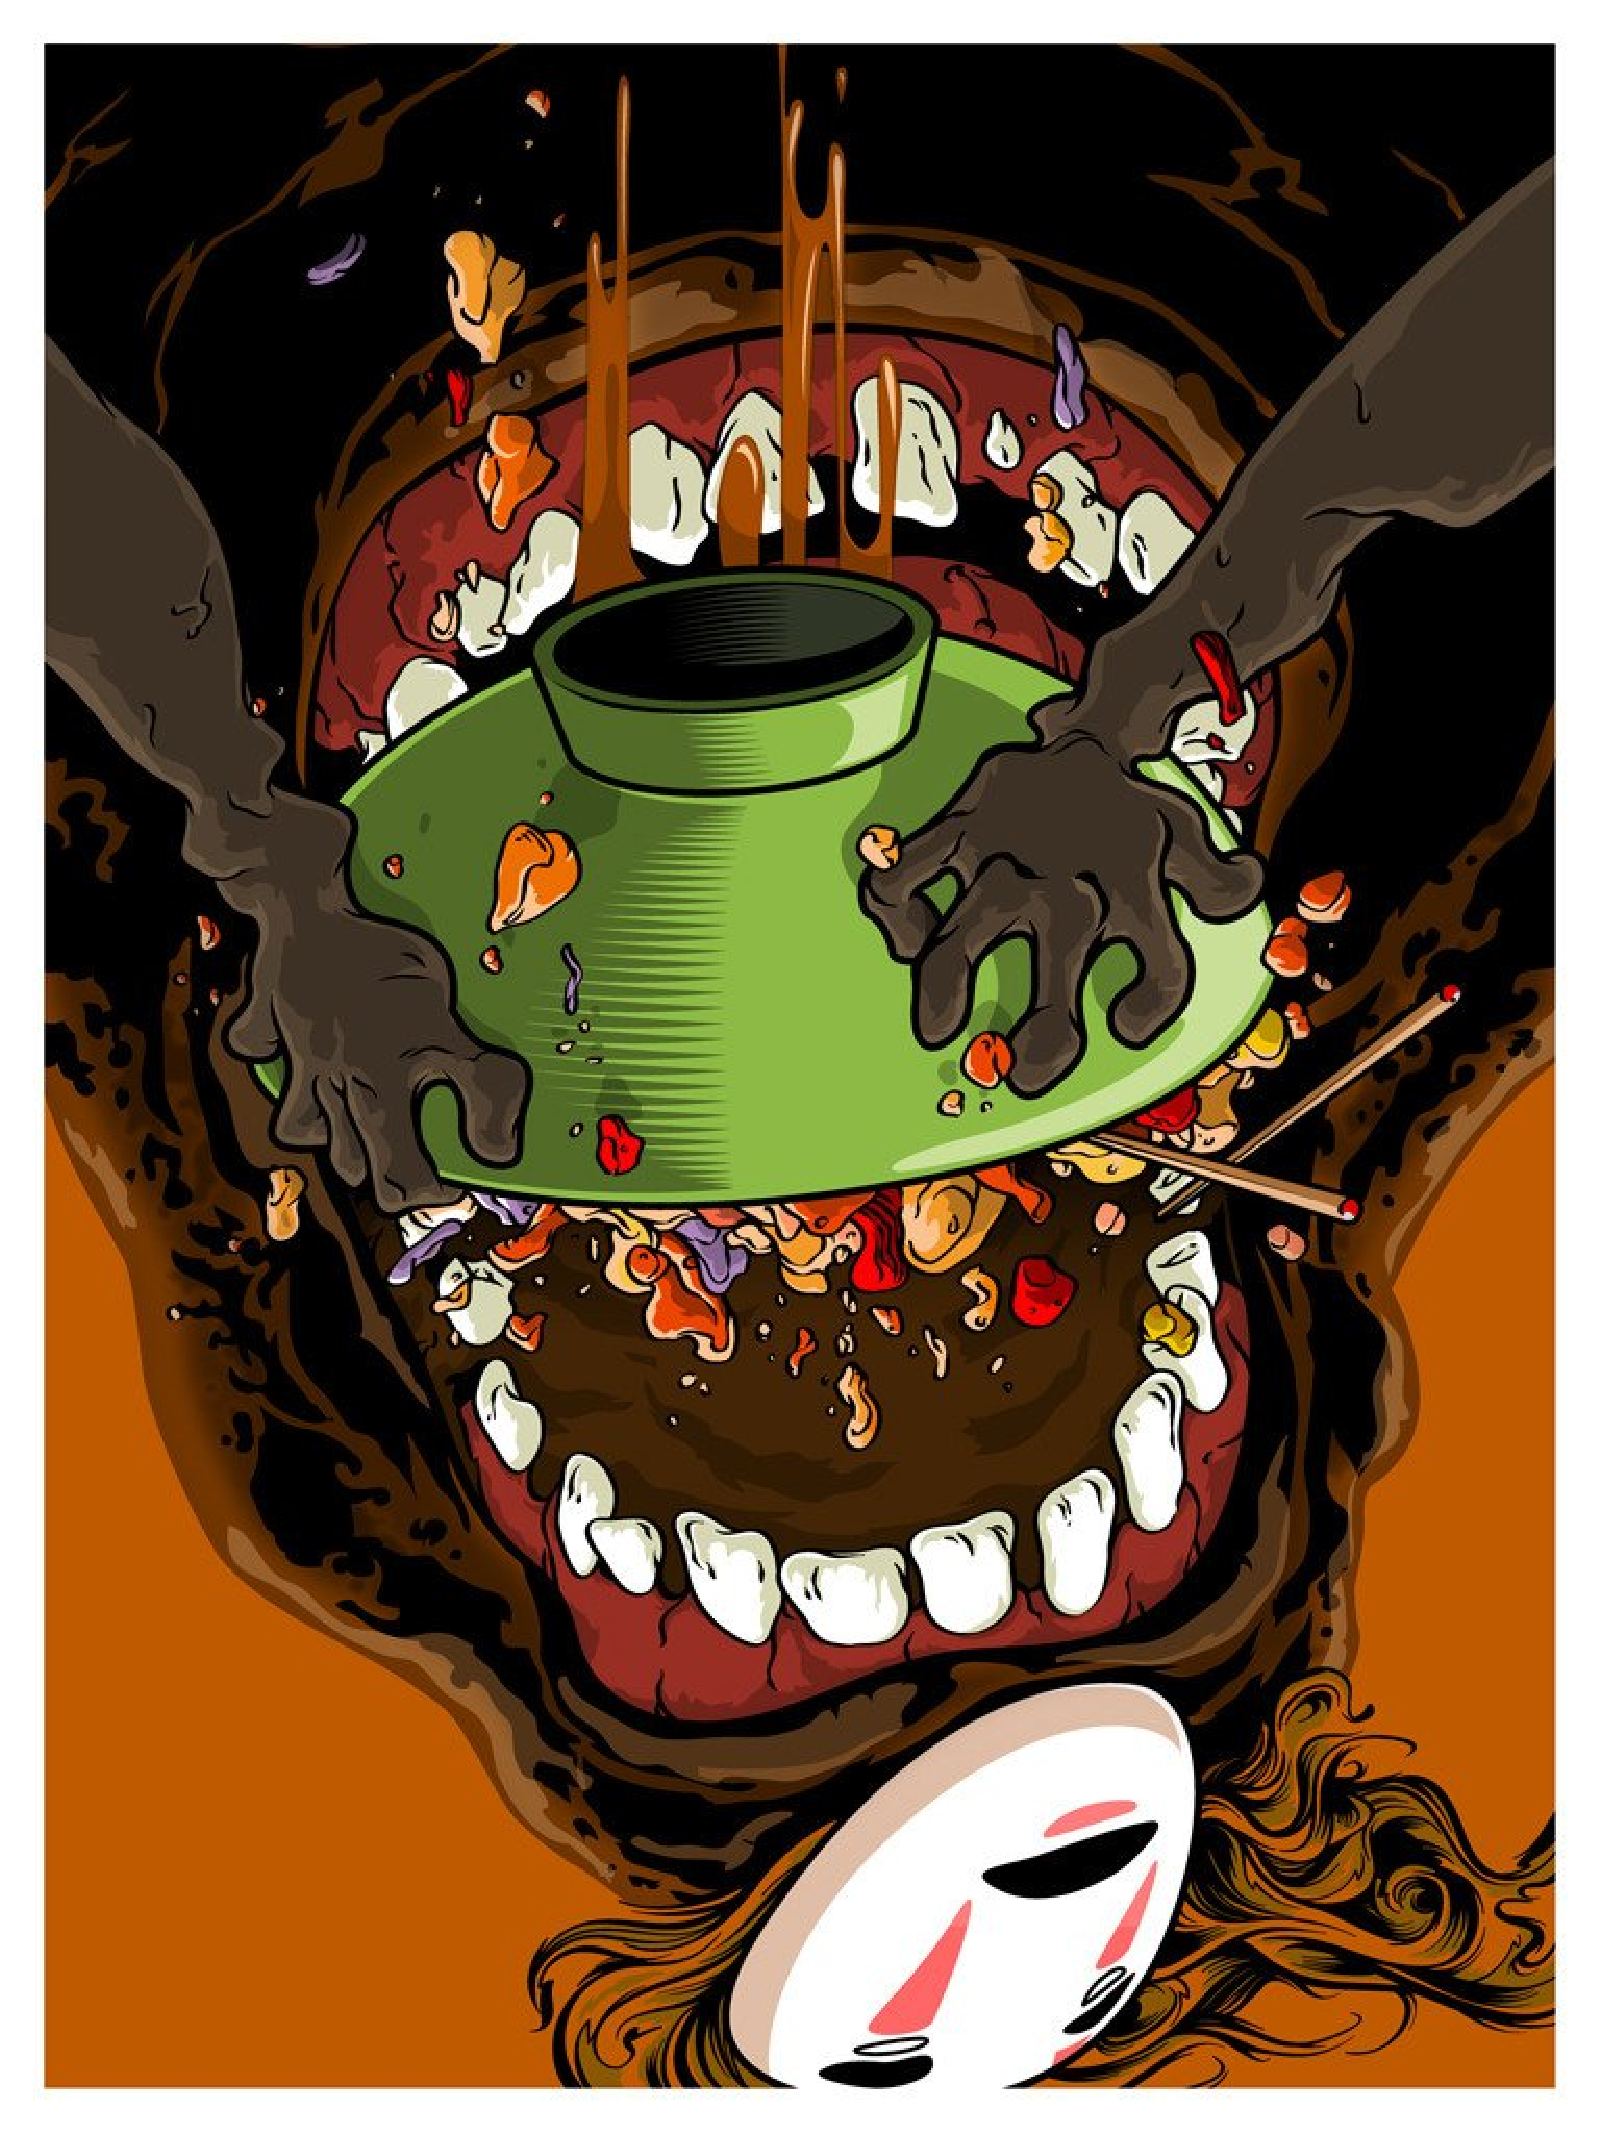
\includegraphics[width=1\linewidth]{pop6}
   \end{turn}
 \end{minipage}
 \caption{Это что, поп-арт?}
\end{figure}

\end{document}